% asset_id: FAS2EulerianTraversabilityAndRouteInspectionTikZ-001
% asset_type: TikZ
% unit_code: FAS2
% topic_code: FAS2-GRAPH
% topic_id: FAS2EulerianTraversabilityAndRouteInspection
\documentclass[tikz,border=8pt]{standalone}
\usetikzlibrary{positioning,calc}
\begin{document}
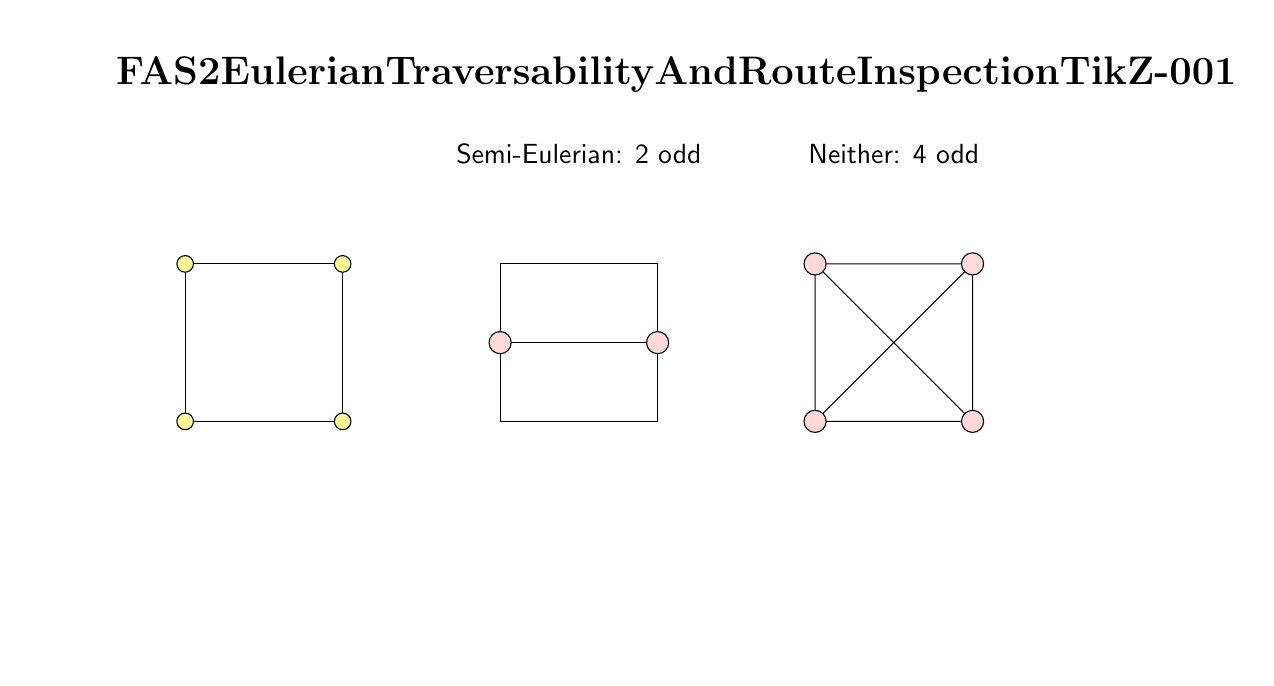
\begin{tikzpicture}[font=\sffamily]
\fill[white] (-1,-1) rectangle (13,7);
\node[anchor=west,font=\bfseries\Large] at (0,6.4) {FAS2EulerianTraversabilityAndRouteInspectionTikZ-001};


ode at (2,5.4) {Eulerian: 0 odd};
\draw (1,4) -- (3,4) -- (3,2) -- (1,2) -- cycle;
\foreach \x/\y in {1/4,3/4,3/2,1/2}{\filldraw[fill=yellow!40] (\x,\y) circle (3pt);}
\node at (6,5.4) {Semi-Eulerian: 2 odd};
\draw (5,4) -- (7,4) -- (7,2) -- (5,2) -- cycle (5,3)--(7,3);
\filldraw[fill=red!15] (5,3) circle (4pt); \filldraw[fill=red!15] (7,3) circle (4pt);
\node at (10,5.4) {Neither: 4 odd};
\draw (9,4)--(11,4)--(11,2)--(9,2)--cycle (9,4)--(11,2) (11,4)--(9,2);
\foreach \x/\y in {9/4,11/4,11/2,9/2}{\filldraw[fill=red!15] (\x,\y) circle (4pt);}

\end{tikzpicture}
\end{document}
